%%%%%%%%%%%%%%%%%%%%
%%%%%%%%%%%%%%%%%%%%
%%
%% Andrea Tino - 2019
%% Programming + Science
%% Opinion model
%%
%%%%%%%%%%%%%%%%%%%%
%%%%%%%%%%%%%%%%%%%%

\section{Developing a CA to describe people's opinion change}
\label{sec:opinionca}

In section \ref{sec:simpleca}, we have built our first automaton: Conway's Game of Life.
That CA is a great start because it has many interesting configurations and evolutions;
however, now, we want to move forward and develop another, different, automaton.
A CA is a mathematical model; other than being a very funny thing to play with, it is a
tool that can be used to study our reality from a theoretical perspective. Like any other
model, it is capable of simplifying our universe so that we can study specific things
about a natural phenomenon. CGL was just an automaton we built without a specific goal
in mind, we just wanted to play with automata!
For the next stage, we want to build a CA that can help us reach a distinct objective:
analyzing opinion change among the members of a society.

\subsection{Working out the model}
We want to use a scientific approach to solve a problem. So, 
before going straight to coding, we need to:

\begin{enumerate}
\item Decide what natural phenomenon we want to describe and control. 
We basically want to answer the question: what is the problem we want to solve?
\item Define the mathematical model to reach that objective. We 
basically need to translate
our problem into mathematical terms. This step is called: \textit{modelization}.
\item Create a computer simulation by translating into code the mathematical
model we created, this stage is called: \textit{simulation}. While simulating,
it is possible to collect all sorts of data and measurements; those will be used
to rate which model best achieves the objectives with \textbf{highest performance} and
\textbf{lowest cost}.
\item After all simulations have been run, the best model is selected and then
effectively put in practice. Most of the times, it results in something being
physically built, or a process being enforced. This stage is called:
\textit{implementation}.
\end{enumerate}

% Figure
%
\begin{figure}[b]
\centering
\sidecaption
% tikz diagram
%
% Tikz Diagram
%

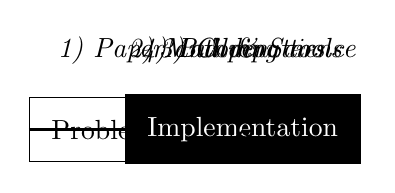
\begin{tikzpicture}

%\pgfdeclareimage{bulb}{assets/light-bulb}

\tikzmath{
	\x = 3.4;
    \sx = \x + \x;
    \ssx = \sx + \x;
    \y = -0.75;
}

\node[draw,inner sep=8pt] (prob) at (0,0) {Problem definition};
\node[draw,inner sep=8pt,fill=gray,text=white] (mod) at (\x,0) {Modelization};
\node[draw,inner sep=8pt,fill=black,text=white] (sim) at (\sx,0) {Simulation};
\node[draw,inner sep=8pt,fill=black,text=white] (impl) at (\ssx,0) {Implementation};

\draw[->,draw=black,thick] (prob) to (mod);
\draw[->,draw=black,thick] (mod) to (sim);
\draw[->,draw=black,thick] (sim) to (impl);

%\node {\pgfbox[center,bottom]{\pgfuseimage{bulb}}};

\node at (0, \y) {\textit{1) Paper and pen}};
\node at (\x, \y) {\textit{2) Math \& Science}};
\node at (\sx, \y) {\textit{3) Computers}};
\node at (\ssx, \y) {\textit{4) Building tools}};

\end{tikzpicture}

%
% If not, use
%\picplace{5cm}{2cm} % Give the correct figure height and width in cm
%
\caption{Illustration of the different phases in the scientific approach to solve a problem.
Each one of them is executed with different tools and require different skills.}
\label{fig:sciappr}
\end{figure}
%

This way of doing things (visualized in figure \ref{fig:sciappr})
is called: \textit{scientific approach} and is at the very core
of what scientists, mathematicians and engineers do every day. So let's start
with the first step: what problem do we want to solve?

\begin{proposition}[Problem definition]
\label{prop:opinionproblem}
Consider the community of people inside a city. The city council has set a goal to reduce
the amount of cars, plastic and pollution on the whole urban area with the intention of
promoting sustainability, green resources, and renewable energies.

The city administration, however, does not have much money to enforce the new green policies
it wants, so it has to rely on the citizens to try to adopt a more green and sustainable life
in complete autonomy. So they have hired us, a group of scientists, to find a solution to
this problem.
\end{proposition}

Proposition \ref{prop:opinionproblem} seems quite tough right? We now are scientists and we
have been given the job to try to convince the inhabitants of a whole town to change their
daily lives and habits to be more green and sustainable (using less plastic, riding bikes instead of
cars, trashing fewer objects, etc.). How are we going to do that?
For starters, no panic! We have an approach to follow, so let's use the method pictured in figure
\ref{fig:sciappr} to solve our problem.\\

Where are we in that diagram? We have passed the first stage, as we now know what problem we must focus
on. So, now it is time to think about the solution and we do that by using Mathematics and Science. What we
want to study is basically a population made of different individuals: men, women and children.
The city council wants us to find a way to persuade the citizens to change their lifestyle. Changing
a person's behavior or habits means to change their opinion on specific matters. No, we are not talking
about \textit{Inception}\footnote{A sci-fi/thriller movie released in 2010 where a group
of people attempts to plant an idea inside a man's mind by violating his dreams. 
If you haven't seen
it, you should because it's pretty cool: \url{https://www.imdb.com/title/tt1375666/}.}, we want to
use less drastic/invasive (and more legal) strategies. One common way of doing this is by
running an \textit{advertising campaign} with TV spots and street cartboards to promote
the concepts we want. However, remember that we don't have much money, so we cannot run these ads all
over town as it would be too expensive: we have a \textbf{limited budget}, which means we can only run
\textbf{small local campaigns} in blocks or areas of the city. Would this strategy suffice?\\

From different social studies, like mentioned by Flache et al. \cite{flache-opinion},
it has emerged that people change their opinion also in relation to
the community where they live. Try to think about one time where your opinion about something shifted,
and try to recall what caused that change: most likely it was because you met and talked with another
person about that subject and the conversation made you change your mind. All that being said,
of course folks' opinion doesn't vary so quickly with just one interaction, it depends
on which person we meet, and what topic we are focusing on. Also, people are very different: some
change opinion quite easily, while others are much more stubborn.

However, here's the most important point, no matter how easily a person's opinion change, what matters
is that it can actually change and the change is caused by the opinions of other individuals. It's like
if opinions were contagious to a certain extent. So, since we cannot run a town-wide ad campaign, we can
rather do the same but in a few areas of the city to change a few people's mind
about sustainable lifestyle so that they will later influence their neighbors. But how many citizens
do we need to convince, so we have enough of them to guarantee their opinion will successfully spread
across the whole town?
Should we run a bigger campaign on a single city block? Or smaller campaigns in more different areas
of town? Or some other strategy?
To answer that question, we are going to use... you guessed it: a CA!\\

To use a CA for our problem, we need to create one, so we must define its properties:

\begin{enumerate}
\item \textbf{What do the cells represent?} A cell represents a single individual (citizen) in the city.
A cell's neighborhood represents the people that live close to that person
(same building, same city block, etc.).
\item \textbf{What is the state of a cell?} Every individual (cell) can be either: \textit{convinced}
($1$, active, black), or \textit{unconvinced} ($0$, inactive, white) about sustainable lifestyle.
\item \textbf{How do we define the state transition function?} The main idea is that a non-convinced citizen
would become convinced if there is a sufficient number of his neighbors that are already convinced.
Of course the opposite applies as well: if a great number of his neighbors is not convinced,
a convinced individual will also turn unconvinced.
\end{enumerate}

We have the basics of our CA, but we need to work more on the transition function. If we read again the
last point in our list above, we can express with simple mathematical expressions what we wrote:

\begin{proposition}[Opinion shift CA transition function]
\label{prop:opicatrans}
Given a cell $y_{i,j} \in E$ in our opinion analysis CA, its next state is defined by this
transition function:
\begin{equation}
f(n) =
  \begin{cases}
    0       & \quad n < N^\ast\\
    1       & \quad n \geq N^\ast\\
  \end{cases}
\end{equation}
Where $n = 0 \dots 8$ is the number of active neighbors of $y$, and $N^\ast = 0 \dots 9$ is a threshold
value.
\end{proposition}

As you can see from proposition \ref{prop:opicatrans}, transition function $f$ uses a value $N^\ast$ to
set a point where a citizen changes his mind, this number is quite important:

\begin{definition}[Turning Point]
\label{def:tp}
When the transition function $f$ is defined as per proposition \ref{prop:opicatrans}, then quantity
$N^\ast$ is called: \textit{Turning Point} (TP).
If at least $N^\ast$ neighbors are convinced about
a topic, then a citizen would turn or remain convinced too, while if the number of convinced neighbors
is below that value, then a citizen would turn or remain unconvinced.
\end{definition}

Let's talk a bit more about the TP.

\begin{proposition}[Meaning of the Turning Point]
The TP, as per definition \ref{def:tp}, is a quantity and a parameter of our model which,
depending on its value, can describe different important behaviors of individuals in the population,
as shown in table \ref{tab:meaningn}.
\end{proposition}

%
% Table
%
\begin{table}[!t]
\centering
\caption{Showing the meaning of TP $N^\ast$ in relation to the behavior of individuals
in the population.}
\label{tab:meaningn}
%
% Follow this input for your own table layout
%
\begin{tabular}{p{0.15\textwidth}p{0.25\textwidth}p{0.5\textwidth}}
\hline\noalign{\smallskip}
Range of $N^\ast$ & Meaning & Description \\
\noalign{\smallskip}\svhline\noalign{\smallskip}
$N^\ast = 0$ & Stubbornly convinced & No matter what his
neighbors think, this person will never ever turn unconvinced.\\
$1 \leq N^\ast \leq 2$ & Easy to convince  & Such a person does not
require many neighbors to change his feelings about the topic.\\
$3 \leq N^\ast \leq 5$ & Reasonable/average & It takes a fair
intermediate amount of neighbors to make him change his mind.\\
$6 \leq N^\ast \leq 8$ & Hard to convince & A fairly high amount of
neighbors is required to convince people like this to shift their opinion.\\
$N^\ast = 9$ & Stubbornly unconvinced & No matter what his
neighborhood thinks about the topic, this citizen would never ever turn convinced about it.\\
\noalign{\smallskip}\hline\noalign{\smallskip}
\end{tabular}
\end{table}
%

So, we can choose to create a CA where all the citizens have a certain value of $N^\ast$, and
we could create different scenarios where citizens are easy to convince or hard to do so.
By inspecting the evolution of the CA, we would know how to create small ad campaigns to ensure
that the highest possible number of citizens can become convinced about sustainable lifestyle.

\subsection{Building the automaton}
Now it's time to jump on stage 3 of figure \ref{fig:sciappr}. We can finally start coding to
create this new CA. Of course we are not going to reinvent the wheel and start from scratch: we
have already created an automaton: CGL, so let's start from that project and modify a few things.
It turns out that not much code needs to be written to edit CGL and turn it into this new
automaton we want to build now.

\begin{enumerate}
\item Go to the folder containing our project directory \texttt{cellautom}.
\item Duplicate directory \texttt{cellautom} and name the clone: \texttt{opinionca}.
\item From now on, work inside \texttt{opinionca}.
\end{enumerate}

We have basically duplicated CGL and prepared a copy of it that we will edit. In fact, now we must
make a few adjustments in code to develop a different automaton. The first thing, being the title
of the page:

\begin{programcode}{index.html (snippet)}
Open \texttt{index.html} and change the title as shown below.
\begin{codehtml}
<title>Opinion Shift Study Cellular Automaton</title>
\end{codehtml}
\end{programcode}

This was an important step! Now let's move on to some more serious coding.

\begin{programcode}{ca.js (snippet)}
Open \texttt{ca.js} and spot function \texttt{calculateState}. Remove the content of the
function and place this code instead.
\begin{codeh1}{1}{9}
function calculateState(state, neighSum) {
  const N = 3; // Turning Point

  if (neighSum > N) {
    return 1;
  } else {
    return 0;
  }
}
\end{codeh1}
\end{programcode}

We have re-written function \texttt{calculateState}, which is, basically, the state
transition function in code. Now we have a completely different set of rules and this is
not CGL anymore. We have completed coding the first prototype of a
\textit{threshold-based opinion automaton}\footnote{The complex name indicates the way
our automaton describes the opinion of individuals in a population: by using a threshold that we
have called \textit{Turning Point}. In this automaton, a cell changes state when the number
of active neighbors exceeds a certain threshold, that is: $N^\ast$.}.

\subsection{Running simulations}
In our plan (visualized by figure \ref{fig:sciappr}), we are still in stage 3. We have just built
a simulation program (our web application) which runs a CA to describe opinion change in a
city. Now what we need to do is to use this simulator and run it to produce some data. The data
we collect is going to give us the information we want to learn new things that we can use to reach
our goal (as per proposition \ref{prop:opinionproblem}). How do we use the CA? As we have learnt
so far, we need to set different initial conditions and see how the CA evolves.

\begin{proposition}[Simulation strategy]
\label{prop:simstrat}
Given our objective in proposition \ref{prop:opinionproblem}, we want to try to run an ad
campaign on a targeted small set of communities in town, to meet the low budget. We want to try
different configurations of \textit{short-range local campaigns} in the city,
and see how the opinion changes with time. We will select the configuration which ensures
maximum coverage as the automaton evolves.
\end{proposition}

What do we mean by running \textit{short-range local campaigns}?

\begin{itemize}
\item \textbf{Short-range:} An ad campaign will involve few people in a precise area of the city.
\item \textbf{Local:} The community which is targeted by an ad campaign will be covered 100\%, it
means that there will be no individual in the community who won't be exposed to the campaign.
\end{itemize}

The two points explain that, basically, in our CA,
a targeted community will be a \textbf{small} surface (short-range) of black cells
\textbf{without white holes} inside it (local). If we follow this simulation strategy as per proposition
\ref{prop:simstrat}, we basically need to experiment with some initial conditions consisting of small
black areas located on the city territory. We need to find the best arrangement of black areas that
ensures the CA will evolve to a configuration with the highest amount of black cells in the end.
So this is what we are going to do:

\begin{enumerate}
\item Set an initial configuration for the CA, with some small black areas located in
different parts of the grid.
\item Make the CA evolve until a final or recurrent configuration is reached.
\item Take note of the percentage of black cells in the automaton after its evolution. We will call this
measure: \textit{coverage ratio} or \textit{coverage percentage}.
\item Start again trying a different configuration.
\end{enumerate}

At the end, we will compare all the coverage percentages, and we will pick the initial condition
associated to the highest coverage percentage. That initial configuration will be the best
advertising strategy to reach our objective and solve the problem.

\subsubsection{Experimenting a little}
The only requirement is to use small black areas when setting the initial configuration, so
we can have many different possibilities. To avoid making many attempts, we can try to perform
a few simple experiments to see how the CA we built behaves, so that, later, we can try some more
specific initial conditions and save a lot of time.

The first thing we wanna do, is changing the size of our automaton.

\begin{programcode}{ca.js (snippet)}
In \texttt{ca.js}, at the beginning of the module, change the size of the CA to 40x40.
\begin{code}
const rowsnum = 40;
const colsnum = 40;
\end{code}
\end{programcode}

We need a big automaton to describe a city, we cannot use a 9x9. Feel free to use a 
larger\footnote{Be careful. As you will probably see if you set a very big size, the CA gets slower when computing the next configuration when pressing the "Next" button. That is because our code for calculating the next configuration
(function \texttt{next}) performs a number of operations which grows with the number of cells.
The more the CA grows, the slower it gets. This characteristic is also called:
\textit{algorithmic complexity} and we will talk about it in the next chapters.} grid if
you want, however we recommend to have a minimum size of 40x40.\\

We will need to create small surfaces of active cells, we think that drawing small rectangles
is probably the best option to model a local city block or set of apartments. 
From now on, we will refer to a rectangle of black (active) cells as a \textit{block} of cells.
And we are going to draw many blocks. Instead of manually creating a block by filling the
\texttt{initConfig} constant array, which can be tedious, we want to create a function
to which we provide the top-left corner cell and the bottom-right corner cell's coordinates, and it
will push all the cells inside these boundaries into the array \texttt{initConfig}.

\begin{programcode}{ca.js (snippet)}
In our Javascript module, add this function at the beginning, after the constants and variables.
\begin{codeh2}{0}{2}{4}{8}
const initConfig = [];

let t = 0; // Cycles (time)

function setInitialCondition() {
    // In this function, we will populate array 'initConfig'
}
\end{codeh2}
Also note that we have removed any initial value in array \texttt{initConfig}, which now is set
to an empty value at the beginning.

Then, go at the bottom of the module, and insert the highlighted line.
\begin{codeh1}{8}{10}
window.addEventListener("load", function () {
  if (rowsnum < 9 || colsnum < 9) {
    throw new Error("The CA must be at least 9x9.");
  }
  if (cellsize < 4) {
    throw new Error("Cells are too small. A cell must be at least 4px!");
  }

  setInitialCondition();
  create();
  initializeGrid();
  initializeButton();
  updateCycleText();
});
\end{codeh1}
\end{programcode}

What we have done is adding another step in our CA \textit{initialization sequence}. As you can see from
the last snippet of code, we invoke function \texttt{setInitialCondition} right before everything
else. This function, which we will implement in a moment, will populate array \texttt{initConfig}
in a smarter way.

The next thing we need is a quick way to draw a rectangle as we mentioned before. We will create
a function to accomplish that.

\begin{programcode}{ca.js (snippet)}
Add this function in the Javascript module right after function \texttt{setInitialCondition}.
\begin{code}
function rect(i1, j1, i2, j2) {
  // Must: 0 < i1 < i2 < rowsnum AND 0 < j1 < j2 < colsnum
  for (let i = i1; i <= i2; i++) {
    for (let j = j1; j <= j2; j++) {
      initConfig.push(i + ":" + j);
    }
  }
}
\end{code}
\end{programcode}

Function \texttt{rect} will push inside \texttt{initConfig} all the cells that fall inside the
boundaries defined by point \texttt{i1:j1} and \texttt{i2:j2}. The code is quite simple, we have
the usual double scanning of the cells of the automaton; however this time we scan the rows between
\texttt{i1} and \texttt{i2} and the columns between \texttt{j1} and \texttt{j2}, instead of
spanning the whole grid. Also notice the comment: it clarifies that the four cell coordinates
passed as input must respect some conditions: basically the two pairs of coordinates must define
two cells inside the grid; also, cell \texttt{i2:j2} must be placed below and on the right
of \texttt{i1:j1}.
Let's see this new tool in action and let's draw a square block in the automaton.

\begin{programcode}{ca.js (snippet)}
Remove the comment inside function \texttt{setInitialCondition} and
invoke function \texttt{rect}.
\begin{codeh1}{1}{3}
function setInitialCondition() {
  rect(3, 3, 5, 5); // 3x3
}
\end{codeh1}
\end{programcode}

If you save and refresh, you will see that a black square has been set as initial condition,
and that this block starts from cell \texttt{3:3} until cell \texttt{6:6} (3x3).
The size of the drawn rectangle is: \texttt{(i2-i1+1):(j2-j1+1)}.

We want to experiment a little and see what happens to square blocks of different sizes when
the CA evolves. So let's paint a few more blocks of different dimension and let's draw some
conclusions.

\begin{programcode}{ca.js (snippet)}
Add more invocations to function \texttt{rect} inside function \texttt{setInitialCondition}.
\begin{codeh1}{1}{8}
function setInitialCondition() {
  rect(3, 3, 5, 5); // 3x3
  rect(3, 15, 6, 18); // 4x4
  rect(3, 30, 7, 34); // 5x5
  rect(20, 3, 25, 8); // 6x6
  rect(20, 15, 26, 21); // 7x7
  rect(20, 30, 27, 37); // 8x8
}
\end{codeh1}
\end{programcode}

If you refresh the page, you will see our six squares on the grid. Now we go ahead and make the
CA evolve by using the button we developed, and see the result after a few cycles (no more than 5
are really needed). What do we see? The 3x3 square has disappeared completely and the other
squares have just slightly changed shapes but they then remained unchanged.
We can draw the first important learning point here:

\begin{proposition}[Minimum size for alive blocks]
\label{prop:minsizedie}
A block of size $W \times H$, whose shortest dimension is lower or equal than 3: $\min(W,H) <= 3$,
disappears as the automaton evolves.
\end{proposition}

Proposition \ref{prop:minsizedie} draws some more generic conclusions on rectangles instead of squares.
But it is of course valid on squares too, in that case the width and height are always the same so
the proposition reads for square blocks smaller than 3x3, as we witnessed.

\begin{problem}
\label{prob:blocksizedie}
Provide evidence that proposition \ref{prop:minsizedie} is correct by using rectangular blocks
of different sizes instead of squares.
\end{problem}

We have our key learning, so what do we make out of it? Is proposition \ref{prop:minsizedie} a good
finding or a bad one? Think a little about it. We want to create a configuration with small blocks
that will hopefully cause the CA to evolve in a way such that these blocks grow in cycles. But
proposition \ref{prop:minsizedie} has just shown that blocks either shrink and stay or shrink and
disappear. This is not a good finding unfortunately!
So, let's pause and reflect: we know the behavior of
\textit{isolated blocks} now, but why does that behavior occur?

Remember our transition function:
an individual turns convinced only if he has at least 3 convinced neighbors.
Inside a block there are two distinct forces that take place:

\begin{itemize}
\item An \textbf{expanding force} exercised by the area of contiguous black cells which
try to expand their surface.
\item A \textbf{shrinking force} caused by the border of white cells enclosing the block, they
attempt to reduce the size of the block.
\end{itemize}

A block of
black cells 3x3 is apparently not strong enough and is killed by the outer border of white cells
(the shrinking force is stronger).
But when the size increases to 4 or higher, then the black surface is strong enough to keep its state
and is not affected by the white border (the expanding force equals the shrinking one).
It seems like an isolated block will never create an expanding force which exceeds the shrinking one,
therefore isolated blocks cannot solve our problem as they will never grow.

\begin{problem}
\label{prob:highernblockslive}
Prove that, when the Turning Point is 2 or lower, that is $N^\ast < 3$, then isolated blocks can grow.
What does it mean? What conclusions do you draw out of this evidence?
\end{problem}

\begin{problem}
\label{prob:highernblockslive2}
Prove that, when the Turning Point is 4 or higher, that is $N^\ast \geq 3$, then isolated blocks never grow
but always shrink.
What does it mean? What conclusions do you draw out of this evidence?
\end{problem}

We need to find a different strategy. Our understanding is that, since isolated blocks are not
strong enough to expand, they probably need reinforcement. Therefore, instead of considering isolated
blocks, let's use \textit{connected blocks}. We will now make an experiment and paint two blocks
connected by some cells and see what happens. Again, we do not want to write down one cell at a time
inside array \texttt{initConfig}, as we did for blocks;
we want to create a function that
draws a line of connecting cells from one cell to another to save time and be more efficient
in our experiments (so we have a quick way to draw lines). To achieve this, we need a little bit
of Geometry.\\

We eventually want to draw a line of cells from one cell to another. Let's forget about
automata for a moment and let's consider a 2D plane, and let's say we want a way to find
all the points $P = (p_x, p_y)$ that lay on
the segment between two points $A = (a_x, a_y)$ and $B = (b_x, b_y)$.
That equation is the following:

\begin{equation}
\label{eq:kinemseg}
\begin{cases}
p_x = (1-k) \cdot a_x + k \cdot b_x\\
p_y = (1-k) \cdot a_y + k \cdot b_y
\end{cases}
k \in [0,1]
\end{equation}

Equations \ref{eq:kinemseg} are called: \textit{segment equations}, and they work 
this way: parameter $k$ is used as a tuner to move the resulting
point $P$ from $A$ to $B$.

\begin{example}[Using the segment equations]
\label{ex:kinemseg}
Let's take two points on the plane: $A = (4,6)$ and $B = (8,2)$. Draw a coordinate system
on a paper (a squared one is handy in this context),
pick up a unit for both axis, and draw the points at their coordinates. Now draw an arrow
connecting $A$ to $B$ making sure the head points to $B$. Equations \ref{eq:kinemseg}
become:
\begin{equation*}
\begin{cases}
p_x = (1-k) \cdot 4 + k \cdot 8\\
p_y = (1-k) \cdot 6 + k \cdot 2
\end{cases}
k \in [0,1]
\end{equation*}
Let's see how this works. We must use parameter $k$ to get all the points on the segment
connecting $A$ and $B$ (remember that $k$ must be in range: $0 \leq k \leq 1$). If we
start with $k=0$, we get: $P = (4,6) = A$. So at the beginning we start from $A$. If we
set $k=1$, we get: $P = (8,2) = B$. So at the end we get $B$. If everything works the way
it should, if we set $k=0.5$, we expect to get the point which lays in the middle of the
connecting segment. In fact, we have that, for $k=\frac{1}{2}$, $P = (6,4)$; if you draw
this point, you will see it actually sits in the middle of the segment.
If we set $k=\frac{1}{4}$, we get $P = (5,5)$.
If we set $k=\frac{3}{4}$, we get $P = (7,3)$.
As you can see, as $k$ approaches $1$ from $0$, we go from $A$ to $B$ on
the $\overrightarrow{AB}$ vector (directed line).
\end{example}

In example \ref{ex:kinemseg} we had some fun with equations \ref{eq:kinemseg}
and experienced how they work. At this point, we need to adapt those equations to our automaton.
The problem is that, in our automaton, the coordinates are integer numbers, not rational
numbers. What we need to do is called: \textit{approximation}. We need to approximate
the results of equartions \ref{eq:kinemseg} to the closest integer number.
To do that, we just need to apply a \textit{ceiling} function to $p_x$ and $p_y$, so that we get
these equations instead:

\begin{equation}
\label{eq:kinemsegapprox}
\begin{cases}
p_x = \lceil (1-k) \cdot a_x + k \cdot b_x \rceil\\
p_y = \lceil (1-k) \cdot a_y + k \cdot b_y \rceil
\end{cases}
k \in [0,1]
\end{equation}

When we take a number $x \in \mathbb{R}$ and do this: $\lceil x \rceil$, we are calculating
the \textit{ceiling} of that number: we basically approximate $x$ up to the closest integer.

\begin{example}[Understanding numeric ceiling]
If we take $x = 3$, this number is already an integer, so $\lceil x \rceil = \lceil 3 \rceil = 3$.
If we take a rational number like: $x = 3.3$ then we need to pick up the first integer that
comes after that number; that number is $\lceil x \rceil = \lceil 3.3 \rceil = 4$.
Here are a few more examples: $\lceil 0.2 \rceil = 1$, $\lceil 0.001 \rceil = 1$,
$\lceil 0.999 \rceil = 1$, $\lceil 100.1 \rceil = 101$ and $\lceil 5.5 \rceil = 6$.
\end{example}

Now that we have everything we need to draw lines on a squared grid, we can implement
equations \ref{eq:kinemsegapprox} in code.

\begin{programcode}{ca.js (snippet)}
Add this function right after function \texttt{rect}.
\begin{code}
function line(i1, j1, i2, j2) {
  // Must: 0 < i1, i2 < rowsnum AND 0 < j1, j2 < colsnum
  for (let k = 0; k <= 1; k += 0.01) {
    let p1 = (1-k) * i1 + k * i2;
    let p2 = (1-k) * j1 + k * j2;
    p1 = Math.ceil(p1);
    p2 = Math.ceil(p2);
    initConfig.push(p1 + ":" + p2);
  }
}
\end{code}
\end{programcode}

Function \texttt{line} takes 4 arguments: the coordinates of the two cells we want to connect
with a line, that is \texttt{i1:j1} and \texttt{i2:j2}. Note the comment which clearly
describes the acceptable values of the coordinates: this time we just require the coordinates
to be inside the grid size, the cells can be located anywhere in the automaton. Let's try our
new function.

\begin{programcode}{ca.js (snippet)}
Remove the content of function \texttt{setInitialCondition}, and invoke function \texttt{line}
instead.
\begin{codeh1}{1}{3}
function setInitialCondition() {
  line(3, 3, 10, 30);
}
\end{codeh1}
\end{programcode}

If we save and refresh, we will see our line.
So, let's test our theory about connected blocks. Let's now draw two squares and a line connecting
them to see if the number of black cells increases this time.

\begin{programcode}{ca.js (snippet)}
Remove function \texttt{setInitialCondition}'s content again, and create two blocks and one
line connecting them.
\begin{codeh1}{1}{5}
function setInitialCondition() {
  rect(2, 2, 6, 6); // 3x3
  rect(20, 15, 26, 21); // 7x7
  line(5, 5, 20, 15);
}
\end{codeh1}
\end{programcode}

As you can see, we have created the line to start from the lower-right corner of the top square to
the top-left corner of the bottom one. Let's refresh and see our initial state: now two blocks
are connected via a thin line of cells. If we try to advance by one cycle in the evolution, we
unfortunately see that the line almost immediately disappears and, as we move on with cycles,
the two blocks (which get isolated) will change shape recurrently but will not expand. The line
is not strong enough, we need a thicker one.

\begin{programcode}{ca.js (snippet)}
Add this line of code inside function \texttt{line}.
\begin{codeh1}{8}{10}
function line(i1, j1, i2, j2) {
  // Must: 0 < i1, i2 < rowsnum AND 0 < j1, j2 < colsnum
  for (let k = 0; k <= 1; k += 0.01) {
    let p1 = (1-k) * i1 + k * i2;
    let p2 = (1-k) * j1 + k * j2;
    p1 = Math.ceil(p1);
    p2 = Math.ceil(p2);
    initConfig.push(p1 + ":" + p2);
    initConfig.push(p1 + ":" + (p2+1)); // Thick line
  }
}
\end{codeh1}
\end{programcode}

The line we added will make sure that, for every cell \texttt{p1:p2}
we add in the initial configuration, we also add
the cell on its right: \texttt{p1:(p2+1)}. Let's try again in the browser to make the CA evolve
now that the connecting line is evidently thicker than before.
Eureka\footnote{Typical expression mathematicians use when they get at the bottom of
a problem and find a solution. This expression was in fact used the first time by Archimedes
to celebrate a discovery or invention.}! We can finally see that the black surface expands
gradually and, after 18 cycle, the automaton stabilizes onto a final configuration where we have
more black cells than when we started.

\begin{proposition}[Expanding initial configurations]
\label{prop:expinitconfig}
Basing on our experiments, we could assess that the initial configurations that seem to generate
a black surface expanding evolution are those where there are small active connected blocks.
\end{proposition}

\subsubsection{Trying out different initial configurations}
Basing on the findings from our investigations, as per proposition \ref{prop:expinitconfig}, we
now have a strategy. We have discovered that small connected black blocks will expand into wider
black surfaces, which is exactly the effect we want here. So, now the question is about understanding
what specific initial configurations (respecting the characteristics we described in
proposition \ref{prop:expinitconfig}) we should use to get the best result in achieving a solution
to the problem in proposition \ref{prop:opinionproblem}.

\begin{proposition}[Simulation objective]
\label{prop:simobj}
We want to find the initial condition (or the set of initial conditions, if more can be found)
that causes the opinion-shift automaton to evolve into a configuration with the
highest possible number of active cells, starting from the fewest possible number of active ones.
\end{proposition}

Let's start with a first attemp: let's create two small blocks at the opposite corners of the city
and let's connect them with a line.

\begin{programcode}{ca.js (snippet)}
Remove function \texttt{setInitialCondition}'s content again, and create two blocks and one
line connecting them.
\begin{codeh1}{1}{5}
function setInitialCondition() {
  rect(3, 3, 7, 7); // 5x5
  rect(33, 33, 37, 37); // 5x5
  line(6, 6, 33, 33);
}
\end{codeh1}
\end{programcode}

If you try to make the automaton evolve, you will see that we achieve a quite interesting
expansion after 25 cycles, and then the automaton does not change anymore. However the
final extension of the black surface is not that high. The wider the two blocks, the wider the
final surface, but we cannot make the two blocks too big otherwise we exceed the
budget (remember that we are trying to solve the problem as specified in proposition
\ref{prop:opinionproblem}).\\

Let's try another configuration: we can still work with two blocks, but we will try to make them a
bit bigger (not too much though to avoid exceeding the budget).

\begin{programcode}{ca.js (snippet)}
Remove function \texttt{setInitialCondition}'s content, and create two blocks of different size and one
line connecting them.
\begin{codeh1}{1}{5}
function setInitialCondition() {
  rect(3, 3, 17, 7); // 15x5
  rect(27, 33, 37, 37); // 11x5
  line(6, 6, 35, 35);
}
\end{codeh1}
\end{programcode}

When the CA evolves, this condition will stabilize into a final configuration with a pretty well
extended black surface. It also seems like, if the blocks get wider in one direction
(higher width, or higher height), the final result is also better. However, the problem is always the same:
we cannot create blocks that are too wide.\\

Let's attempt one configuration more. Maybe if we used more blocks connected together we could achieve
our goal. Let's now create an initial condition with four blocks at the corners connected with
an \texttt{X} pattern.

\begin{programcode}{ca.js (snippet)}
Remove function \texttt{setInitialCondition}'s content, and create four blocks and two
lines connecting them.
\begin{codeh1}{1}{7}
function setInitialCondition() {
  rect(3, 3, 7, 7); // 5x5
  rect(3, 33, 7, 37); // 5x5
  rect(33, 33, 37, 37); // 5x5
  rect(33, 3, 37, 7); // 5x5
  line(6, 6, 33, 33);
  line(7, 34, 33, 7);
}
\end{codeh1}
\end{programcode}

As the automaton evolves now, we can see that, after some cycles, the final black surface practically covers the whole
grid. All cells, inside the area defined by the four initial squares, eventually turn black.

\begin{proposition}[A solution to the problem]
\label{prop:sol}
In order to solve the problem described in proposition \ref{prop:opinionproblem}, we have assessed that an
initial configuration of peripheral, small, black blocks connected in a way that the lines cross the whole grid
passing through the center, actually allows the automaton to evolve into a final configuration where all the cells
inside the region delimited by the initial blocks turn black. If the initial blocks are placed as close to the border
of the grid as possible, then the final black area will span all the automaton's cells (border excluded).

In terms of our problem, it means that we need to run small intensive ad campaigns in local peripheral neighborhoods
of the city, making sure that we also run micro-campaigns in city blocks connecting these neighborhoods passing through
the city center.
\end{proposition}

\begin{problem}
\label{prob:opinionproof1}
In the CA we have built, try an initial configuration with 4 small peripheral blocks connected by 4 lines that
run along the border and do not pass through the center. How does the automaton evolve?
\end{problem}

\subsection{Drawing conclusions}
Proposition \ref{prop:sol} provides a possible solution to the problem we formulated in proposition \ref{prop:opinionproblem}.
But it is probably not the only one. Maybe more solutions exist. If they do, it could be nice to understand which of
the solutions we found is the best; one way to assess this is by:

\begin{enumerate}
\item Evaluating the total number of cells that turn black in the end. The initial condition that makes the CA
evolve into a final configuration with the highest number of black cells wins.
\item If more different initial conditions are able to generate a final black surface with the same number of black cells,
then their \textit{speed} can be evaluated. We need to measure the number of cycles that were necessary for the CA to
reach the final configurations starting from each of those initial conditions. 
The fastest (the one that causes the CA to reach
the final configuration with the least number of cycles) wins.
\end{enumerate}

We encourage you to experiment more and investigate the existence of other solutions. Also try to play with the
Turning Point $N^\ast$ and experiment with stubborn populations ($N^\ast > 6$).
